
\chapter{Evaluation}
\label{sec:evaluation}
% \begin{itemize}
% \item measurement setup / results / evaluation / discussion
% \item whatever you have done, you must comment it, compare it to other systems, evaluate it
% \item usually, adequate graphs help to show the benefits of your approach
% \item each result/graph must not only be described, but also discussed (What's the reason for this peak? Why have you observed this effect? What does this tell about your architecture/system/implementation?)
% \item recommended length: approximately one third of the thesis.
% \end{itemize}

\section{Methodology}
One challenge in programming the controller and the WESs,
is the state-based approach and the fact that the WESs can only communicate restricted with each other.
There were therefore two types of state machines, one for the controller and one for the WESs.

The testbed \cref{fig:testbed} is set up so that the PC is connected to the microcontroller 
via wired \ac{UART}, this microcontroller is the controller.
The controller communicates exclusively via ESP-NOW with the WESs,
these then control in different ways with the stage lights and motors.
The WESs never respond to the controller for the actual application, the communication is unidirectional.
However, in order to evaluate the test data, 
the WESs are put into a mode in which they send the data back to the controller via ESP-NOW.
From there, the controller sends it back to the PC via UART.

\begin{figure}[h]
	\centering
	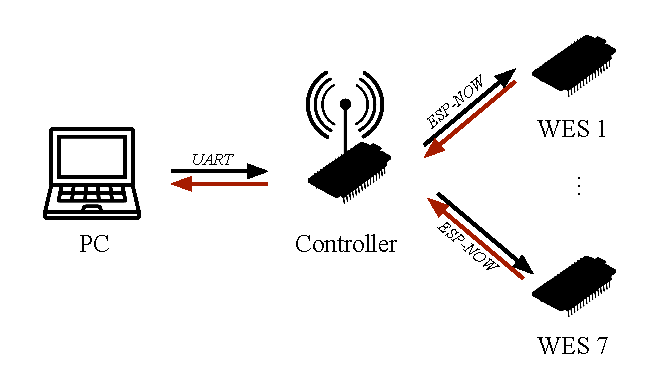
\includegraphics[scale=0.75]{figures/TestFlow.pdf}
	\caption{Data Flow for Measurement}
	\label{fig:testbed}
\end{figure}

The experiment is started from the PC, a JSON is then transmitted to the controller via \ac{UART} using a Python script.
The JSON contains all the parameters that are needed to carry out a test.
At the time the JSON string is transmitted, the controller should be idle so that the packet is read correctly.

\begin{table}[h]
	\centering
	\begin{tabular} { lll }
	\toprule
	\multicolumn{1}{c}{Variable}
	& \multicolumn{1}{c}{Example}
	& \multicolumn{1}{c}{Explaination} \\
	\midrule
	VERBOSE               & 0 				& Enable VERBOSE \\
	DEBUG                 & 0 				& Enable DEBUG \\
	TIMESTAMP\_UART       & 0				& Enable UART timestamps \\
	SEQUENCE\_REPETITIONS & 200				& Sequences per experiment \\
	FULL\_REPETITIONS     & 1000			& Repetitions of the experiment \\
	MASTER\_CHANNEL       & 6				& Wi-fi Channel of the Controller \\
	WES\_CHANNEL          & 6				& Wi-fi Channel of the WES \\
	WAIT\_AFTER\_SEQ      & 0				& delay between sequences \\
	WAIT\_AFTER\_REP\_EXP & 2000			& delay between experiments \\
	IS\_BROADCASTING      & 1				& BC:=1, UC:=0 \\
	RAPID\_REPETITIONS     & 2				& BC: Rapid Repetitions \\
	CHANNEL\_TOTAL        & 160	 			& BC: Addressed Payload \\
	BROADCAST\_FRAME\_SIZE& 200 			& BC: Maximum Payload/Brodcast \\
	UNICAST\_FRAME\_SIZE  & 20				& UC: Payload/Unicast \\
	WES\_COUNT            & 6				& UC: WES Count \\
	AIRTIME               & 0				& Capture airtime\\
	\bottomrule
	\end{tabular}
	\caption{JSON Experiment Setup}
	\label{tab:json}
\end{table}

When the controller has received its JSON, it must go through three states, 
regardless of further input from the PC shown in \cref{fig:sequenceDiagram}.
\subsubsection*{Setup}
After the start-up, the controller waits for a JSON. When the JSON is received, it sets the corresponding variables.
It then forwards these to the individual WESs using unicast. 
To be absolutely sure that the respective WES has received the setup information,
the number of retransmits in the application layer is set to infinity.
It distributes the data round-robin, the MAC addresses of all WESs are hardcoded, but could also be transmitted via JSON.
If the first byte of the setup unicast is set to 253, the WES knows that it is a metadata packet and handles it accordingly in its callback function.
\subsubsection*{Testing}
When the controller has ensured that each WES has received the measurement data, it starts transmitting the dummy test data.
Sequences are then sent according to the variable SEQUENCE\_REPETITIONS.
The duration varies greatly depending on the number of sequences and the protocol used.
\subsubsection*{Collecting}
When the controller has processed all sequences, it makes a request to one of the WESs, 
again with the help of a 100\% reliable unicast forced on the application layer.
This then transmits the measured values and in turn ensures that these have also arrived at the controller.
The measured values are then transmitted to the PC and the experiment is repeated until the required number of experiments has been completed.

\begin{figure}[h]
	\centering
	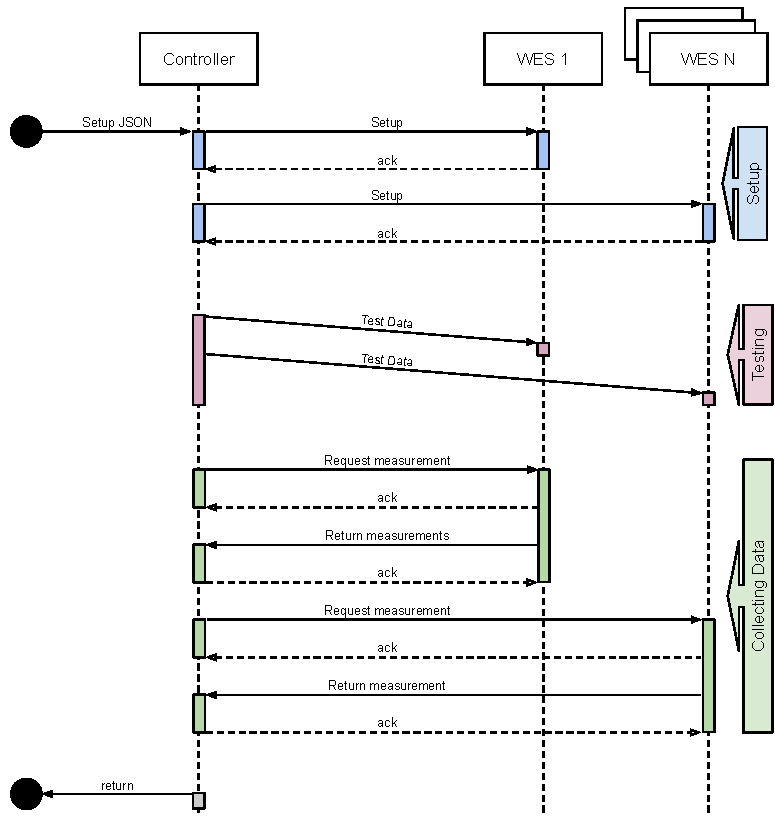
\includegraphics[scale=0.9]{figures/sequence_diagram_drive.pdf}
	\caption{Sequence Diagram of the measurment and data collection}
	\label{fig:sequenceDiagram}
\end{figure}

\section{Wireshark's measurements}

The Wireshark tool is suitable for recording traffic.
In order to record packets outside a LAN, the WI-FI card must be set to monitor mode.
In this mode, frames from an ad-hoc network can also be sniffed, as is the case with ESP-NOW.
\cref{fig:wiresharkUC} shows how each unicast is followed by an acknowledgement, 
as mentioned in \cref{sec:unicast}

\begin{figure}[h]
	\centering
	\includegraphics[scale=0.5]{figures/wiresharkUC.pdf}
	\caption{Unicast Transmissions Recording from Wireshark}
	\label{fig:wiresharkUC}
\end{figure}

The data frame \cref{fig:wiresharkUCTransmission} displays the measured airtime of 696$\mu$s.
In the calculation from \cref{tab:airtime_unicast_calc}, however, it was only 536$\mu$s.
Adding the average backoff of a free channel (160$\mu$s) and the DIFS (50$\mu$s) gives 906$\mu$s.
Wireshark also recognises the category code of the Vendor Specific Action Frame that ESP-NOW uses.
The payload of 20 bytes assumed for unicast in the experiment is given here as 31 bytes,
presumably it has to do with the implementation of the action frame shown in \cref{fig:esp_now_vendor_format}.

\begin{figure}[h]
	\centering
	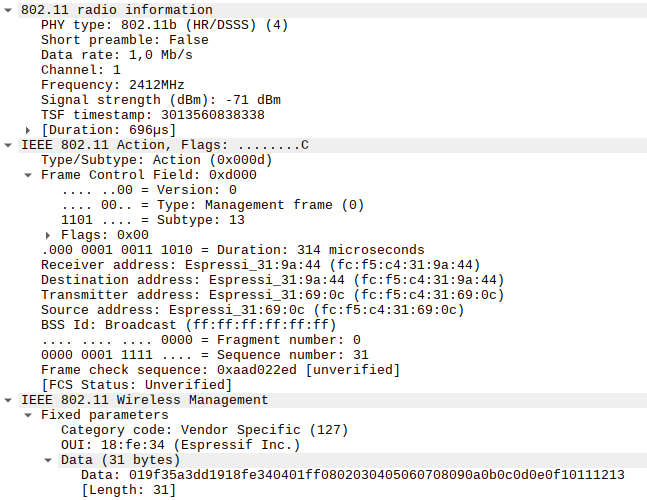
\includegraphics[scale=0.4]{figures/wiresharkUCFrame.png}
	\caption{Unicast Transmission Radio Information from Wireshark}
	\label{fig:wiresharkUCTransmission}
\end{figure}

\href{lst:callback}
A look at the 31 byte "payload" shows that ESP-NOW specific parts of wireshark have not been parsed correctly.
From the representation in \cref{fig:esp_now_frame_format} and \cref{fig:esp_now_vendor_format} 
it can be deduced:

The first 4 bytes of the payload are still the random values and, according to Espressif, 
do not belong to the Vendor Specific Content.
These 4 bytes together with the following 1 byte (Element ID), 1 byte (length) - identified as 25 bytes instead of 20,
Organisation Identifier (3 bytes), Type (1 byte) and Version (1 byte) make up the difference of 11 bytes to the actual payload.
The real payload is filled with the self defined flag 0×ff in \cref{lst:callback} followed by the sequence number 0×00.
The rest of the payload is filled with numbers, which are set to the value of the position in the payload 0×02, 0×03, .., 0×13.

\begin{figure}[h]
	\centering
	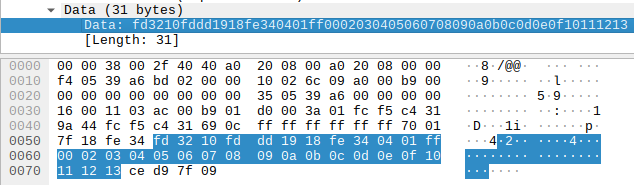
\includegraphics[scale=0.4]{figures/wiresharkPayload.png}
	\caption{Unicast Payload Analysis with Wireshark}
	\label{fig:wiresharkPayload}
\end{figure}

For completeness, a recording of the broadcast traffic also is displayed.
The difference to the unicast traffic is,
that the destination address is bundled in a transmission of 160 bytes
instead of being distributed in $8 \cdot 20$ byte packets.
As already mentioned, the acknowledgements are not usable with the broadcast.

\begin{figure}[h]
	\centering
	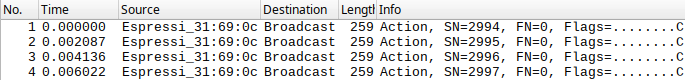
\includegraphics[scale=0.5]{figures/wiresharkBC.png}
	\caption{Unicast Payload Analysis with Wireshark}
	\label{fig:wiresharkBCTransmission}
\end{figure}

\section{Protocols under Study}

\subsection*{Slim Unicast vs Slim Broadcast}

In the design part it became clear that it is much more efficient 
to reach many individual WESs with one broadcast instead of many individual unicasts.
Tracking the transmissions with Wireshark also confirms this assumption in \cref{fig:transmissionTime}.

\begin{figure}[h]
	\centering
	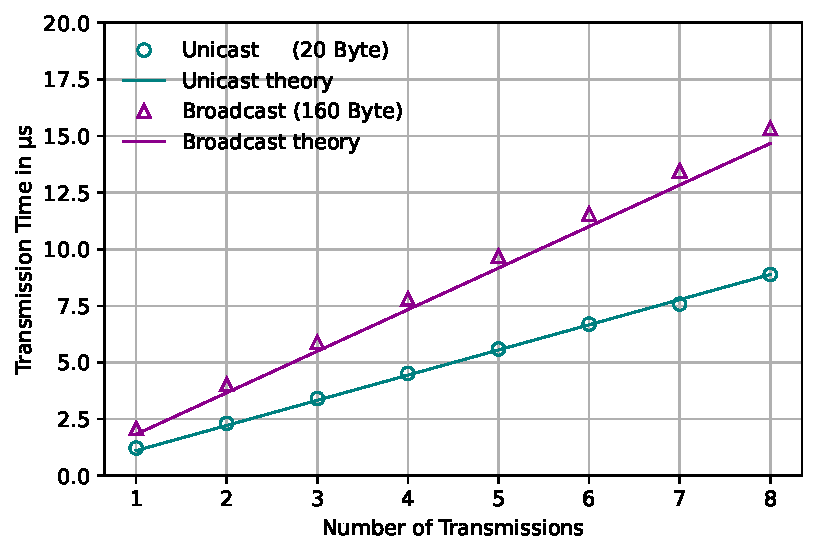
\includegraphics[scale=0.6]{../Plot2/Graphs/bc_uc_transmissiontime_wireshark.pdf}
	\caption{E.g. Transmission Time of Slim Unicast and Slim Broadcast}
	\label{fig:transmissionTime}
\end{figure}

The theoretical assumptions clearly correspond to the measured values,
Additional latencies due to processing in the microcontroller or at the antenna are therefore hardly significant.
The update frequency for the unicast decreases sharply as the number of stations increases,
whereas the broadcast decreases only slowly. 
With unicast, it can be seen that the measured values fluctuate around the values assumed in theory.
This is because these are exemplary values from the Wireshark measurement of \cref{fig:wiresharkUC} 
and these are not averaged over all experiments.
The fluctuation can be explained by the fact that the backoff is randomly selected from the \ac{CW}.
The backoff is randomly selected from the \ac{CW}, thus explaining the fluctuation.
Measurments of the transmission time for broadcasts with smaller payloads were not made.
Therefore, a broadcast is clearly superior to an unicast in terms of latency,
update frequency and synchronisation.

Slim Unicast can only make a difference through its reliability.
The channel in the experiment was free, so no retransmissions had to be sent, which would have delayed the transmission time even more.
When implementing slim unicast, it makes sense to do so without synchronisation, because the buffering delay would be too long.
However, it is also difficult to estimate how many transmissions can be saved if only changed values trigger a transmission.
But it makes sense to simulate a stress test because critical errors become apparent precisely
when packets are lost and all values are changed.

It can be said that Slim Broadcast is the superior design due to the much lower part of overhead, 
because the data throughput is significantly higher.
The WESs can also be synchronised more easily because the transmissions reach many people at the same time.
The weak point, however, is reliability.

\subsection*{Rapid Repetition}

The Success Ratio, which is calculated from the number of successfully received packets 
and the total number of packets sent, demonstrates a good metric to measure reliability.
In the test setup of 8 distributed WESs, some placed close to the controller, 
some at a slightly greater distance,
this naturally varies greatly as shown in \cref{fig:sr_broadcast}.
The measurement was carried out in my flat distributed over different rooms.
Several WLANs use the same 2.4 GHz band and lead to indifferences.
For the slim broadcast, 160 byte packets were distributed in 600 sequences and 
the experiment was repeated 1000 times.

\begin{figure}[h]
	\centering
	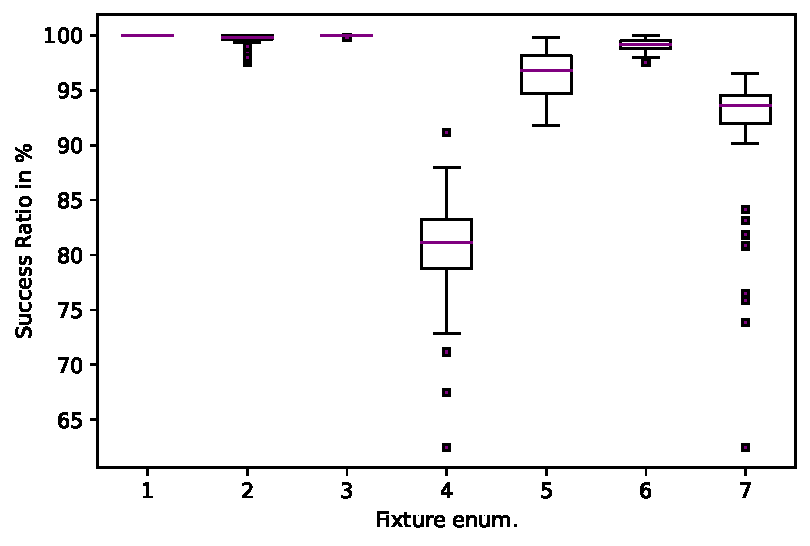
\includegraphics[scale=0.6]{../Plot2/Graphs/SR_per_fixture_broadcast.pdf}
	\caption{SR of Broadcasts for 7 WESs}
	\label{fig:sr_broadcast}
\end{figure}

The before discribed experiment shows that especially WES4 and WES7 have poor reception,
while the reception of other WESs is much better.
WES1, WES2 and WES3 where in the same room as the controller, 
WES1 in particular was only a few centimetres away from the transmitter and actually has no packet loss.
With the Slim Unicast 100\% of the packets arrived and there was no loss of data.
One approach to improve reliability at the expense of latency was rapid repetitions.

With RR, it must be weighed up how many repetitions are sensible, 
because at some point the performance beyond reliability is impaired too much.
WES4 has the weakest reception and is supposed to represent a kind of worst-case scenario.

\begin{figure}[h]
	\centering
	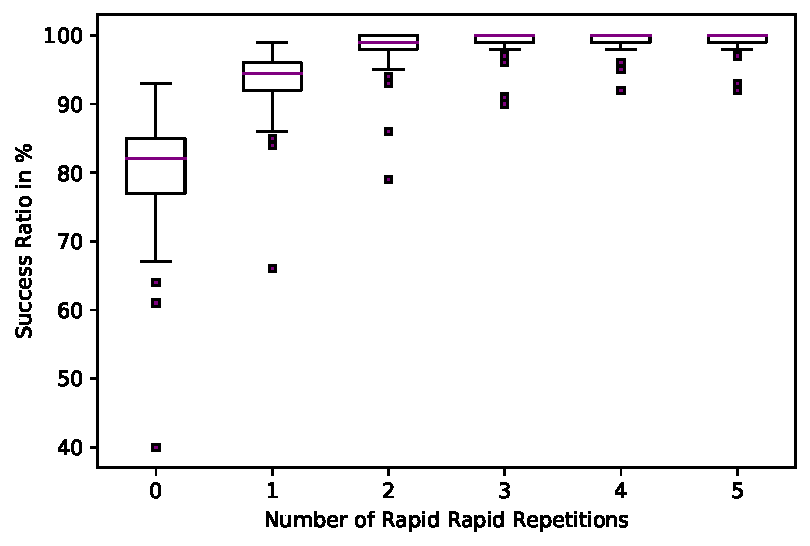
\includegraphics[scale=0.6]{../Plot2/Graphs/SR_of_node4_rr.pdf}
	\caption{SR of WES4 with altered RRs}
	\label{fig:sr_broadcast_wes4}
\end{figure}

It becomes clear that even a few repetitions lead to a significantly better SR,
but it is no longer improved as much after two repetitions (RR=2).

\begin{figure}[h]
	\centering
	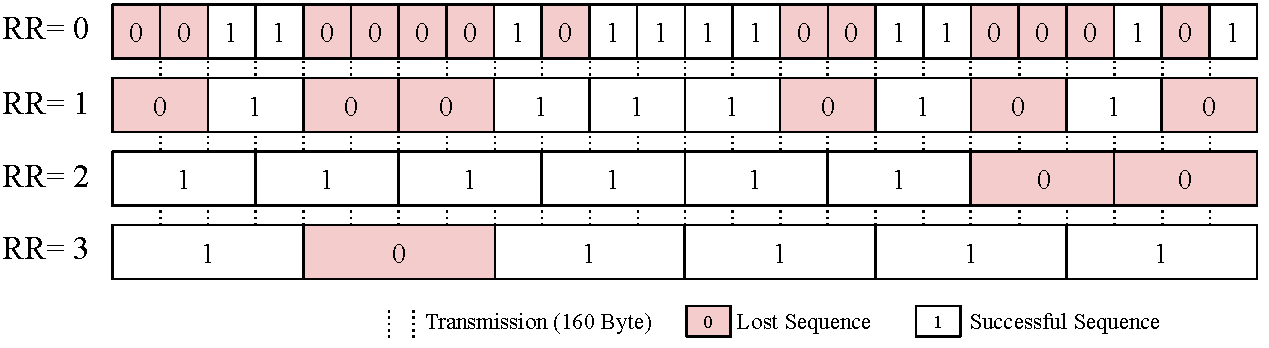
\includegraphics[scale=0.5]{figures/rrBitwise.pdf}
	\caption{Bitwise Example of RR (WES=4, SeqNr.=9-24, ExpNr.=1)}
	\label{fig:rrBitwise}
\end{figure}

However, a reliability of 100\% as with unicast is not necessarily achieved.
A look at the measurement data shows why, illustrated in \cref{fig:rrBitwise}.
The given excerpt is from an actual measurement of the WES4, 
the channel here is bad and causes several bursts of packet loss.
Increasing the repetitions from RR=0 to RR=1, slightly dampes the loss of packets.
However, it is noticeable that even with RR=3,
one sequence is still lost, despite the 4 times costs of latency and throughput.
The problem is that faulty packets often come clustered 
and the repetitions still fall within the range of the bad channel.
It is worth mentioning that individual sequences arrive at RR=2, although they are lost at RR=3.
This can also be seen in \cref{fig:rrBitwise}, 
the second and third sequence of RR=2 get over the channel interference,
whereas the second sequence of RR=3 falls right into the interference and is therefore lost.
Of course, this is rather rarely the case, 
which can be seen in the significantly increased success ratio.

\subsection*{Delayed Repetition}

To circumvent this circumstance, the sequences can be nested in \cref{fig:badChannel},
this is only possible in combination with the Rapid Repetitions.
Subsequently, swapping the sequence numbers makes it possible to make an evaluation on the same data.
WES4 is chosen again because the packet loss is very high.

\begin{figure}[h]
	\centering
	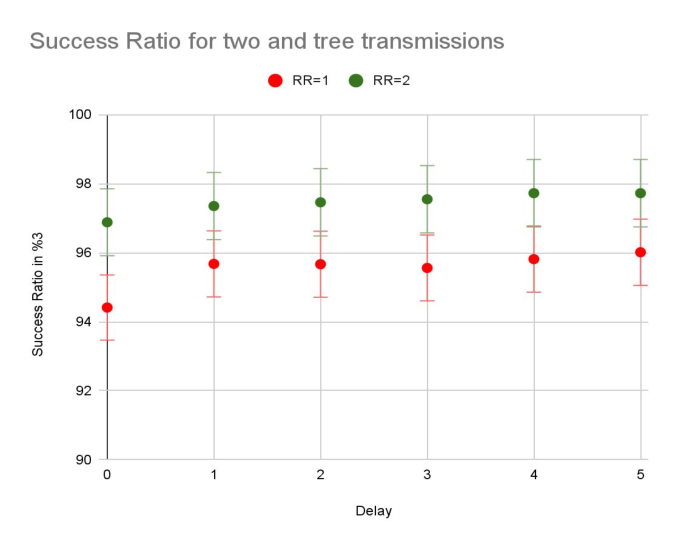
\includegraphics[scale=0.8]{figures/bufferingDelay.pdf}
	\caption{SR for Buffering Delay with/without RR for WES4}
	\label{fig:bufferingDelay}
\end{figure}
\todo{update Graphic!}

In \cref{fig:bufferingDelay} it is quite clear that the success ratio increases the longer the delay of the repetition is.
It can therefore be proofed that the success ratio is noticeably improved with a constant update frequency, 
already with a buffering delay of 1, is the effect significant. \todo{How significant - after the plot is updated, give an exact example}
It also shows that the use of the buffering delay does not improve the success ratio so much 
that one less repetition could be sent.
In addition, the use of buffering delay has a cost in latency, as mentioned in FIGURE. \todo{Link to graphic of buffering delay latency theory}.
It must therefore be weighed up whether the additional latency justifies the increased success ratio.
\todo{Address syncronization problem?}

% TODO
% \subsection*{Impact of Groupsize}

% \todo{optional}
% When controlling lighting installations, the human eye does not notice so clearly 
% if all lights are switched synchronously but with a delay.
% However, it is clearly noticeable when a single light reacts with a delay.
% With the BUffering Delay, synchronisation can be achieved, 
% but what happens if a control signal does not arrive even despite RR and BD?
% In the following, the Success Ratio is only considered successful if the control signals have arrived at all WESs.

% \TODO{optional: SR Figure, different approaches with groupsize of 7, UC, BC, RR=1, RR=1+DR=1 RR=2, RR=2+DR+1, RR=3. RR=3+DR=1, RR=3+DR+2}

% Evaluation \todo{optional: write evaluation}

\section{Results}
% \begin{itemize}
% 	\item Which method had the best results?
% 	\item Tabelle mit allen Protokollen auflisten 
% \end{itemize}

In the measurements, the unicast approach with 20 bytes each or a broadcast with 160 bytes were sent to the 8 WESs.
The metrics latency, update frequency, reliability and synchronisation are compared in \cref{tab:results}.

\begin{table}[h]
	\centering
	\begin{tabular} { llllll }
	\toprule
	\multicolumn{1}{c}{Slim}
	& \multicolumn{1}{c}{}
	& \multicolumn{1}{c}{Update}
	& \multicolumn{2}{c}{Reliability in \%} 
	& \multicolumn{1}{c}{} \\

	\multicolumn{1}{c}{Protocol}
	& \multicolumn{1}{c}{Latency in $\mu$s}
	& \multicolumn{1}{c}{Frequency in Hz}
	& \multicolumn{1}{c}{Average}
	& \multicolumn{1}{c}{WES 4}
	& \multicolumn{1}{c}{Sync} \\

	\midrule
	UC        &  696–59128 & 16–130  & 100.00 & 100.00 & no \\
	UC sync   & 7581–59128 & 16      & 100.00 & 100.00 & yes \\
	BC        &  1816      & 479     & 95.45  & 80.50  & yes \\
	BC 1xRR   &  3903      & 239.5   & 98.37  & 93.51  & yes \\
	BC 2xRR   &  5990      & 159.7   & 99.40  & 98.22  & yes \\
	BC 3xRR   &  8077      & 119     & 99.62  & 99.04  & yes \\
	BC 1xRR+DR&  5204      & 239.5   & 99.03  & 95.79  & yes \\
	BC 2xRR+DR&  8386      & 159.7   & 99.36  & 97.64  & yes \\
	BC 3xRR+DR&  11538     & 119     & 99.68  & 99.20  & yes \\
	DMX (base)&  22700     & 44      & 100.00 & 100.00 & yes \\
	\bottomrule
	\end{tabular}
	\caption{Comparison of the measured results}
	\label{tab:results}
\end{table}
%mastertabelle:

It quickly becomes apparent that the Slim Unicast, both with and without synchronisation, 
is more reliable than the broadcast, but broadcast has a much better latency and update frequencies.
These values become particularly extreme when the lights are to react synchronously.
In the absence of synchronisation, the values vary greatly, 
because the latency varies depending on whether the WES is in the first or last position of the round-robin
and on the number of retransmissions that have to be made if a packet is lost.

With the solutions that use a broadcast, 
it becomes clear that synchronisation between the WESs is deterministically given,
because all WESs receive the signal at the same time.
The difference is mainly due to the DIFS and the backoff 
which have to be waited for before the second repetition can be sent.
But the reliability without RR especially for WES4 is too low (80.5\%).
But the use of rapid repetitions also shows that the reliability of the weaker WES4 in particular is extremely improved.
With 3 rapid repetitions, the reliability reaches a range that is also acceptable for the WES4 (99\%).

Finally, there is the use of delayed repetition (DR) to broadcasts with rapid repetition (RR).
Here, only the delayed repetition with the interlacing of a sequence is shown,
as the effect is greatest here.
It is noticeable that the latency due to the retention of the packets is no longer close to the update frequency, 
as with the other broadcasts, but even higher.
The effect of the delayed repetition fades into the background when the RR is set to 3
and it is more worthwhile to keep the already high latency as low as possible.

Compared with DMX as a baseline, it shows that with this specific setup,
the broadcast is also good with 3 RR, whether with or without DR.
Only the reliability is below that of DMX, and only just,
because even the WES with the worst reception has a success ratio of over 99\%.
The unicast already reaches its limits with this small setup,
even if synchronisation is not taken into account.

\chapter{Conclusion \& Discussion}
% \begin{itemize}
% \item summarize again what your paper did, but now emphasize more the results, and comparisons
% \item write conclusions that can be drawn from the results found and the discussion presented in the paper
% \item future work (be very brief, explain what, but not much how, do not speculate about results or impact)
% \item recommended length: one page.
% \end{itemize}

This thesis introduces various protocols optimised for lighting technology.
These were investigated analytically and experimentally.
A special feature of the protocols is that they send packets on the data link layer
and have additional adaptations in the application layer to improve reliability.

The analytical examination showed that the unicast
scales poorly with many stations,
because the packets only have a few bytes of payload making the overhead too great.
The calculations have shown that even with a few stations, a single broadcast packet
distributes the control signals twice as fast.
In practice, this effect could be even more pronounced,
because an error-free channel without need of retransmissions, was always assumed.

With broadcast, on the other hand, there is no reliability.
The assumptions for the duration of the distribution of all control signals to the stations,
were made with a perfectly clean channel,
but in a realistic scenario, packet loss must be expected.
Rapit repetition in the application layer is intended to counteract this.
By sending the same sequence multiple times, lost packets can be compensated for.
If a long bursts of packet lost is encountered, 
the Delayed Rapid Repetition closes these bursts by staggering the sequences.

The unicast packets arrived successfully at the stations 100\% of the time.
With the broadcast packets, there were significant losses recorded.
It had become apparent that reception was particularly poor at one specific station,
this station was then selected to simulate a bad-case scenario.
The use of rapid repetition led to a significant increase in reliability at this station.
However, up to three retransmissions were necessary to bring the success ratio of the weakest station to over 99\%.
Delayed Rapid Repetitions, with interleaving the sequences, on the other hand, 
had a rather small effect on the success ratio,
especially when many repetitions were sent.
The additional latency caused by the Delayed Rapid Repetition
does not justify the small improvement in the success ratio and is therefore not recommended,
at least for this exemplary setup.
In conclusion, it can be said that 100\% reliability in lighting technology is desirable,
but if the update frequency is high enough,
the next sequence will transmit a new or unchanged control signal shortly afterwards anyway.
A correspondingly high update frequency reduces the influence of missing individual packets.

For the test set-up, a separate procedure protocol was developed,
which should guarantee the smooth running of the test.
One difficulty was to ensure that the stations were always in the correct state.
A controller sent 160 bytes of control information per sequence to 8 different stations.
This was sent either in 20 byte packets as unicast or as a single 160 byte packet as broadcast.
This, of course, corresponds to a very small stage setup.
A DMX Universe is 512 bytes, so it would be interesting to see
how the protocols would behave if they had to distribute the data to 30 stations.
In reality, the size of the control signals of a single station also varies greatly,
which has not been investigated here.

The ESP-NOW protocol was used to implement the transmissions on the data link layer.
A connectionless protocol, which is proprietary, but allows the development of a simple and robust prototype,
originally optimised for low energy.
It only runs on the low-cost platform of the manufacturer Espressif.
It has some limitations that make it difficult to use in practice.
The payload of a transmission may not exceed 250 bytes, 
that if the control signal exceeds 250 bytes, two broadcasts must be sent.
Also limiting is, that no more than 20 stations can be paired with the controller.
Because the protocol only runs on the ESP platform, the transmitter must also be an ESP chip.
This limits the choice of physical layers.
Thus, the behaviour of the 5 GHz frequency band was not investigated.
The test used the outdated IEEE 802.11b protocol, which only works at 1 Mbps,
as the investigation with wireshark prooves.
According to the data sheet, the ESP chip used can achieve data rates of up to 150 Mbps.

The prototype protocols were able to show that transmissions in the data link layer can work properly,
however, tests with larger setups and a non-proprietary protocol are still pending.
